%ekg_7_Diskussion der Alternativen

\subsection{Diskussion der Alternativen}

\subsubsection{Digitale Filterung}

Für die digitale Filterung des Netzbrummens wurden jeweils ein FIR- (Finite-Impuls-Response) und ein IIR- (Infinite-Impuls-Response) Filter als Bandsperren mit einer Sperrfrequenz von \SI{50} {\hertz} entworfen. Hierfür wurden die Filterkoeffizienten mit Matlab erzeugt und danach in C als eigenständige Module implementiert. Die Testung erfolgte auf dem Launchpad des MSP430 mit harmonischen Schwingungen zwischen \SI{1}{\hertz} und \SI{200}{\hertz}, einem künstlichen EKG-Signal (beides mit einer Signalquelle erzeugt) und einem echtem EKG-Signal. 

Der FIR-Filter verfügt zwar über einen linearen Phasenverlauf, erwies sich aber bei den Tests schnell als zu rechenintensiv, für die Anwendung auf dem verwendeten Prozessor. Mit ihm wurde bei einer Abtastfrequenz von \SI{250}{\hertz} lediglich eine Dämpfung von \SI{3}{\decibel} bis \SI{6}{\decibel} erreicht.

Der IIR-Filter zeigte sich im Test mit verschiedenen harmonischen Schwingungen als sehr effizient mit einer maximalen Dämpfung von \SI{150}{\decibel} bei geringem Rechenaufwand. Jedoch führte er in der Anwendung bei einem echten EKG-Signal zu einer Verschlechterung des Ausgangssignals, da er Schwingungen erzeugte, wie aus Abbildung \ref{fig_Test_IIR_Filter} zu erkennen ist. \\

\begin{figure} [h]
	%\centering
	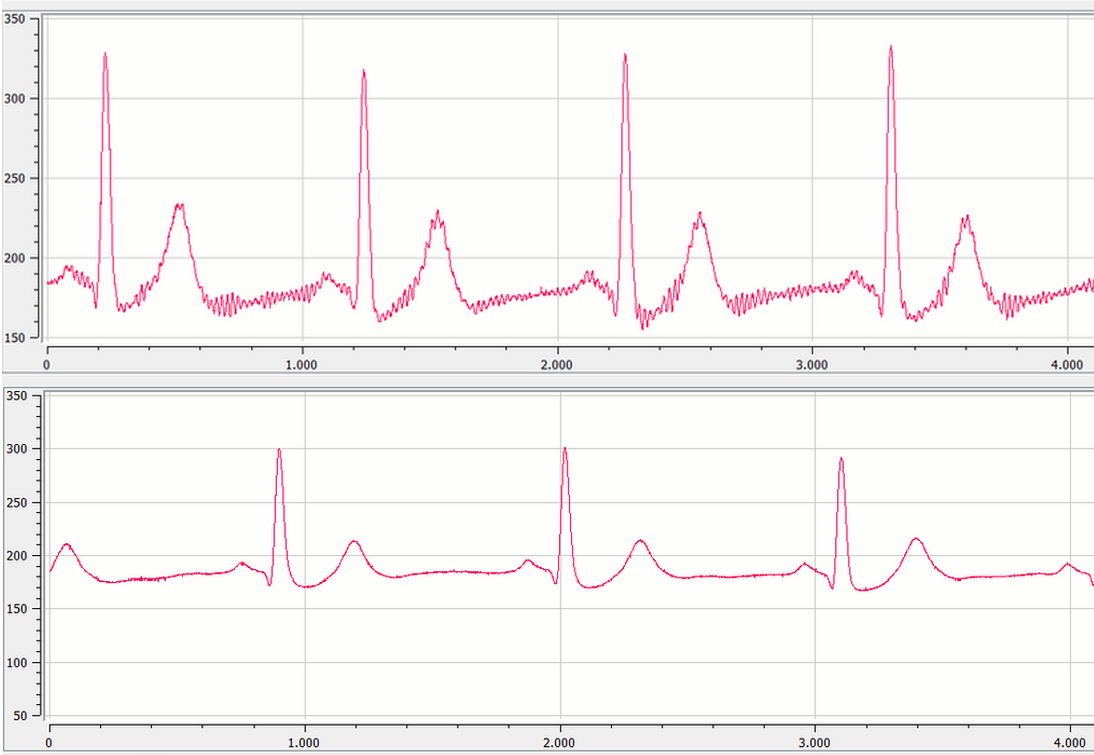
\includegraphics[width=\textwidth] {Test IIR Filter.png}
	\caption{oben: EKG-Signal mit durch IIR-Filter erzeugtes Störsignal; unten: EKG-Signal ohne IIR-Filterung}
	\label{fig_Test_IIR_Filter} 
\end{figure}
%TODO Anhang für FIR und IIR Filter



%TODO PROJEKTGRUPPE: weitere alternative Konzepte die wir ausprobiert oder in Betracht gezogen haben

\subsubsection{Erzeugung der verschiedenen Versorgungsspannungen}

Eine alternative Möglichkeit zur Erzeugung der Unterspannungen ist die Verwendung eines PMIC (Power Management Integrated Circuit), bei welchem es sich um eine integrierte Schaltung handelt, die alle Anfallenden Aufgaben der Spannungserzeugung übernimmt. Dazu zählen: Battery Management (Überwachung des Ladungszustands der Batterie), Spannungsregulation (Bereitstellen von verschiedenen Unterspannungen), Ladefunktionen. Was auf den ersten Blick als gute Lösung für die gegebenen Anforderungen erscheint, gestaltet sich in der praktischen Umsetzung jedoch schwierig. PMICs kommen idr. im QFN48 Package, welches vergleichsweise groß ist und schwierig zu löten. Somit gestaltet sich das Testen einer Schaltung, welche auf einem PMIC basiert als kompliziert. Hinzu kommen die Vergleichsweise hohen kosten des ICs sowie ein hoher Aufwand an externer Beschaltung. Des weiteren bietet ein PMIC wesentlich mehr Features als für die Projektanforderungen nötig wären, weshalb diese Möglichkeit ausgeschlossen wurde.\\